\begin{frame}
\frametitle{Твердотельные накопители (SSD)}
\begin{columns}
  \begin{column}{.5\linewidth}
    Нет подвижных механических частей:
    \begin{itemize}
      \item нет замедления;
      \item хорошо переживают тряску. 
    \end{itemize}
  \end{column}
  \begin{column}{.5\linewidth}
    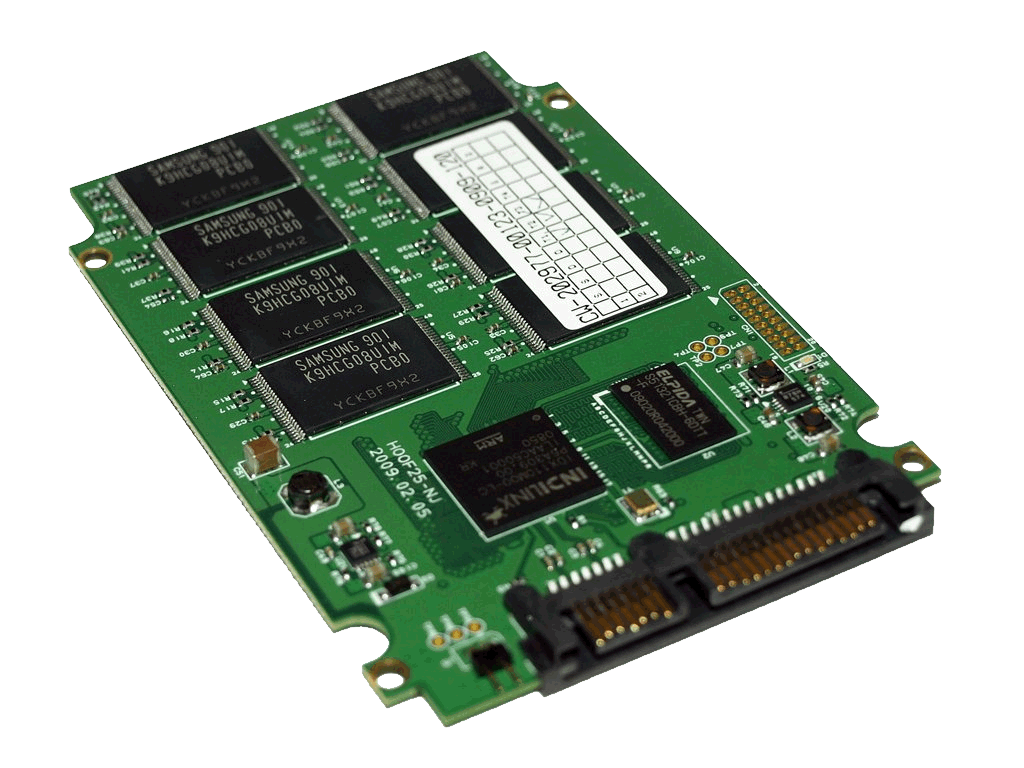
\includegraphics[width=.9\linewidth]{ssd.png}
  \end{column}
\end{columns}
\end{frame}

\begin{frame}
\frametitle{MOSFET}
\begin{center}
  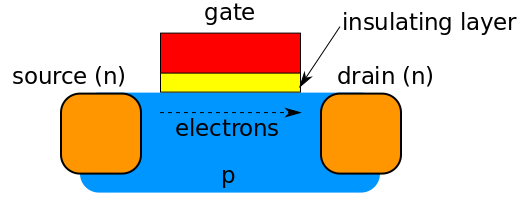
\includegraphics[width=.6\linewidth]{mosfet.png}
\end{center}
\begin{itemize}
  \item В обычных условиях транзистор "заперт":
  \begin{itemize}
    \item даже если между source и drain есть напряжение, тока все равно нет.
  \end{itemize}
  \item Напряжение между source и gate "открывает" транзистор:
  \begin{itemize}
    \item если между source и drain есть напряжение будет и ток.
  \end{itemize}
\end{itemize}
\end{frame}

\begin{frame}
\frametitle{FGMOS}
\begin{center}
  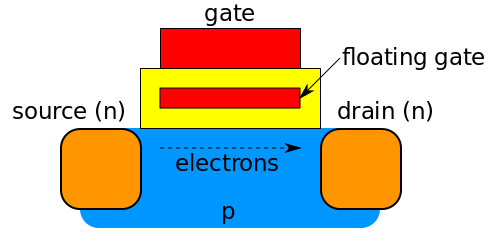
\includegraphics[width=.6\linewidth]{fgmos.png}
\end{center}
\begin{itemize}
  \item MOSFET + дополнительный floating gate:
  \begin{itemize}
    \item floating gate изолирован от всего, но есть способ его зарядить;
    \item floating gate позволяет "нейтрализовать" эффект gate-а.
  \end{itemize}
  \item FGMOS может хранить один бит информации:
  \begin{itemize}
    \item если floating gate заряжен - с FGMOS мы читаем 0;
    \item если разряжен - читаем 1.
  \end{itemize}
\end{itemize}
\end{frame}

\begin{frame}
\frametitle{Изнашивание FGMOS}
\begin{center}
  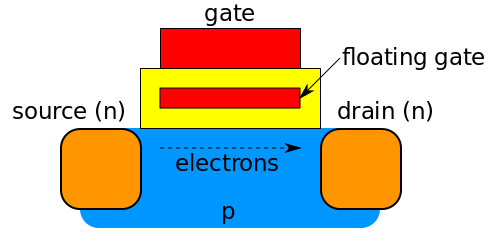
\includegraphics[width=.6\linewidth]{fgmos.png}
\end{center}
\begin{itemize}
  \item Изолятор вокруг floating gate изнашивается:
  \begin{itemize}
    \item чем больше раз запрограмировали/стерли бит хранимый в FGMOS тем
    сильнее изнашивается изолятор;
    \item ячейка памяти с изношеным изолятором становится ненадежной.
  \end{itemize}
\end{itemize}
\end{frame}

\begin{frame}
\frametitle{NAND Array}
\begin{itemize}
  \item FGMOS-ы группируются вместе, чтобы их можно было разместить максимально
  плотно:
  \begin{itemize}
    \item минимальная единица адресации чтения - страница (типично 8-16 Kb);
    \item несколько страниц объединяются в блок - минимальная единица записи
    (типично 32-256 страниц).
  \end{itemize}
  \item При этом SSD диск выглядит как обычный диск, т. е. интерфейс использует
  512 байтные блоки:
  \begin{itemize}
    \item SSD firmware скрывает от нас параметры NAND Array;
    \item firmware следит за тем, чтобы страницы изнашивались равномерно;
    \item для этого внутри SSD работает трансляция адресов + GC + компрессия +
    дедупликация + много других страшных слов.
  \end{itemize}
\end{itemize}
\end{frame}

\begin{frame}
\frametitle{Скорость SSD}
\framesubtitle{Чтение}
\begin{center}
  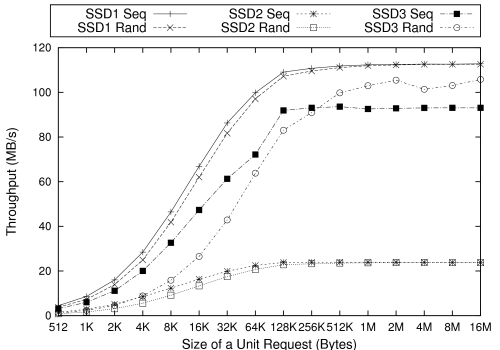
\includegraphics[width=.8\linewidth]{ssd_read_perf.png}
\end{center}
\end{frame}

\begin{frame}
\frametitle{Скорость SSD}
\framesubtitle{Запись}
\begin{center}
  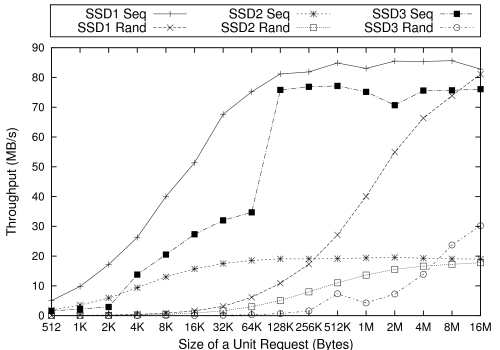
\includegraphics[width=.8\linewidth]{ssd_write_perf.png}
\end{center}
\end{frame}

